\phantomsection
\section*{5. Connectedness and Compactness}
\addcontentsline{toc}{section}{5. Connectedness and Compactness}

\begin{customexa}{c.5.5} Here is some an example for \hypertarget{ex.c.5.5}{\hyperlink{Corollary_5.5}{Corollary $5.5$ (Intermediate Value Theorem)}}.\\
Let $f: S^1 \longrightarrow \R$ be continuous.\\
Claim: such a function can never be injective. (Borsuk–Ulam theorem)\\
Let 
$$g:S^1 \longrightarrow \R, x \mapsto f(x) - f(-x)$$
Note that $g(x) = -g(-x)$. So, $g$ is either the zero function or not.
    \begin{enumerate}
        \item[1)] If $g = 0$, then $f(x) = f(-x)$ for all $x \in S^1$, then $f$ is not injective.
        \item[2)] If $g \neq 0$, then there exists a $x_* \in S^1$ such that 
        \begin{align*}
            g(x_*) > 0 &\text{ or } g(x_*) < 0\\
            \implies g( -x_*) < 0 &\text{ or } g(-x_*) > 0
        \end{align*}
        By the IVT, there exists a $x_0 \in S^1$ such that $g(x_0) = 0$, which means $f(x_0) = f(-x_0)$, that is, $f$ is not injective.
    \end{enumerate}
\end{customexa}

\begin{customexa}{c.5.6} Here are some examples for \hypertarget{ex.c.5.6}{\hyperlink{Corollary_5.6}{Corollary $5.6$}}.
\begin{enumerate}
    \item[1).] $S^1$ is connected: it is the quotient of $[0,1]$ by an equivalence relation $0 \sim 1$.
    \item[2).] The nasty space $\R/\sim$ is connected even not Hausdorff.
\end{enumerate}
\end{customexa}

\begin{customexa}{t.5.7} Here are some examples for \hypertarget{ex.t.5.7}{\hyperlink{Theorem_5.7}{Theorem $5.7$}}.
\begin{enumerate}
    \item[1).] The $2$-sphere $S^2$ is connected:
    $$[0,1] \times [0,1] /_{\partial\left([0,1] \times [0,1]\right)}$$
    \item[2).] The two dimensional torus is connected:
    $$[0,1] \times [0,1] /_{\sim}$$
    \item[3).] The Klein bottle is connected:
    $$[0,1] \times [0,1] /_{\sim}$$
\end{enumerate}
Click here for the amazing drawings of the three (might update later): \href{https://en.wikipedia.org/wiki/Surface_(topology)}{Classification of Surfaces}
\end{customexa}

\begin{customexa}{d.5.3} Here are some examples for \hypertarget{ex.d.5.3}{\hyperlink{Definition_5.3}{Definition $5.3$ (Path Connectedness)}}.
\begin{enumerate}
    \item[1).] $\R^n$ is connected. Let $X = \R^n$, then $X$ is path connected: given $x, y \in R^n$, the function 
    $$f:[0, 1] \longrightarrow \R^n, \,\,\,\, t \mapsto xt + (1-t)y$$
    is a path from $y$ to $x$.
    \item[2).] Let $X = \R^n \setminus \{0\}$. If $n \geqslant 2$, then $X$ is path connected. In pictures:\\
    \begin{minipage}{0.5\textwidth}
        \begin{center}
        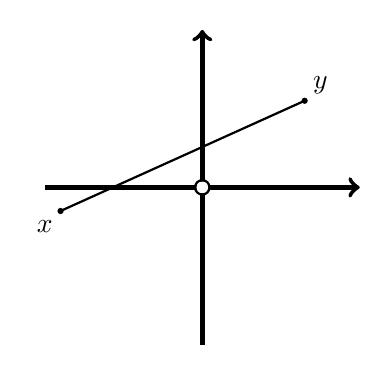
\begin{tikzpicture}[scale = 1]
            \draw[->,ultra thick] (-2,0)--(2,0) {};
            \draw[->,ultra thick] (0,-2)--(0,2) {};
            \node[circle, fill, white, inner sep=1.5pt] at (0, 0) {};
            \draw[black, thick] (0,0) circle[radius=2.6pt];
            \node[label] at (1.5, 1.3) {$y$};
            \node[circle, fill, black, inner sep=0.8pt] at (1.3, 1.1) {};
            \node[label] at (-2, -0.5) {$x$};
            \node[circle, fill, black, inner sep=0.8pt] at (-1.8, -0.3) {};
            \draw[-,thick](1.3, 1.1) -- (-1.8,-0.3);
        \end{tikzpicture}\\
        Case $1$
        \end{center}
    \end{minipage}\begin{minipage}{0.5\textwidth}
        \begin{center}
        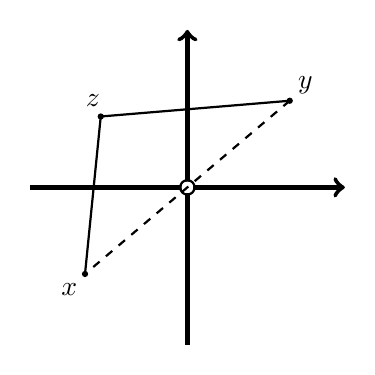
\begin{tikzpicture}[scale = 1]
            \draw[->,ultra thick] (-2,0)--(2,0) {};
            \draw[->,ultra thick] (0,-2)--(0,2) {};
            \node[circle, fill, white, inner sep=1.5pt] at (0, 0) {};
            \draw[black, thick] (0,0) circle[radius=2.6pt];
            \node[label] at (1.5, 1.3) {$y$};
            \node[circle, fill, black, inner sep=0.8pt] at (1.3, 1.1) {};
            \node[label] at (-1.5, -1.3) {$x$};
            \node[circle, fill, black, inner sep=0.8pt] at (-1.3, -1.1) {};
            \node[label] at (-1.2, 1.1) {$z$};
            \node[circle, fill, black, inner sep=0.8pt] at (-1.1, 0.9) {};
            \draw[dashed,thick](1.3, 1.1) -- (-1.3,-1.1);
            \draw[thick](-1.3, -1.1) -- (-1.1, 0.9);
            \draw[thick](-1.1, 0.9) -- (1.3, 1.1);
        \end{tikzpicture}\\
        Case $2$
        \end{center}
    \end{minipage}
    Explicitly in case $2$, $z \in X$ is a point not on the line though $x$ and $y$ and $f$ is the path
    $$f = \begin{cases} x(1-t) + zt &\text{ if }\,\,\, t \in [0,1]\\
    z(2-t) + (t-1)y & \text{ if }\,\,\,
t \in [1, 2]
    \end{cases}$$
    Moral: if $n = 1$, then $X$ is not path connected. Indeed, $X$ has two path components, namely $(-\infty, 0)$ and $(0, \infty)$, so that any path in $X$ has image contained in $(-\infty, 0)$ or $(0, \infty)$. In particular, there is no path from $1$ to $-1$ in $X$.
\item[3).] For each $n \geqslant 1$, the $n$-sphere
    $$S^n = \left\{x \in \R^n \mid ||x||^2 = 1\right\}$$
is (path) connected. Indeed, let $x, y \in S^n$. The great arc from $x$ to $y$ is a path from $x$ to $y$.
\item[4).] Let 
    $$X = \left\{\left(x, \sin{\dfrac{1}{x}}\right)\Big| 0 < x \leqslant 1\right\} \subset \R^2$$
    Then $X$ is (path) connected, being the image of the (path) connected space $(0, 1]$ under the continuous map $\sin{\dfrac{1}{x}}$. The closure $\overline{X}$ is called the {\bf Topologist's Sine Curv e}.
    $$\overline{X} = X \cup \left\{(0, y) \mid -1 \leqslant y \leqslant 1\right\}.$$
    \begin{center}
    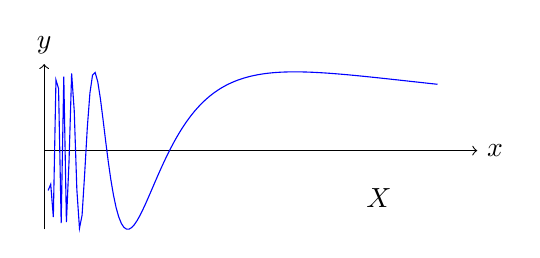
\begin{tikzpicture}[x=5cm]
        \draw[->] (0,0) -- (1.1,0) node[right] {$x$};
        \draw[->] (0,-1) -- (0,1.1) node[above] {$y$};
        \draw[blue,domain=0.01:1,samples=150] plot (\x, {sin((1/\x)r)});
        \node[label] at (0.85, -0.6) {$X$};
        \end{tikzpicture}
        \hspace{0.2cm}
    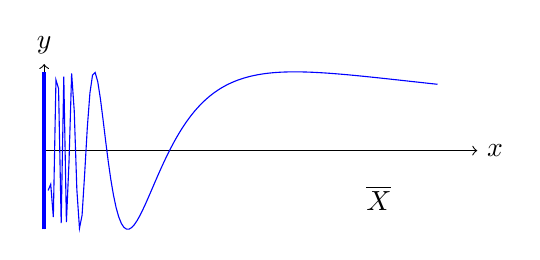
\begin{tikzpicture}[x=5cm]
        \draw[->] (0,0) -- (1.1,0) node[right] {$x$};
        \draw[->] (0,-1) -- (0,1.1) node[above] {$y$};
        \draw[blue,domain=0.01:1,samples=150] plot (\x, {sin((1/\x)r)});
        \draw[ultra thick, blue] (0, -1) -- (0, 1) {};
        \node[label] at (0.85, -0.6) {$\overline{X}$};
        \end{tikzpicture}\\
    (Note: Change the sample size in the \LaTeX\, source to make the graph smoother.)
    \end{center}
    The closure is connected. However, $\overline{X}$ is {\bf not} path connected. Say $f:[0, 1] \longrightarrow \overline{X}$ is a continuous function with 
    $$f(0) = (0, 0), \,\,\,f(1) \in X$$
    Since $A = \{0\} \times [-1, 1] \subset \overline{X}$ is closed, so too is $f^{-1}(A) \subset [0, 1]$. So, $f^{-1}(A)$ has a maximal element, say, $a$. Then $f(a)\in A$ while $f(t) \in X$ if $t > a$.\\
    Write $f$ in components: $f(t) = \left(x(t), y(t)\right)$. Then $x(a) = 0$ and $x(t) > 0$ and $y(t) = \sin{\dfrac{1}{x(t)}}$ if $t > a$. By the condition $x(t) > 0$ if $t > a$, for each $n \geqslant 1$, there exists a 
    $$0 < u < x\left(a + \dfrac{1}{n}\right)$$
    such that $\sin{\dfrac{1}{u}} = (-1)^n$. By the Intermediate Value Theorem, there exists a $0 < t_n < \dfrac{1}{n}$ such that $x(t_n) = u$. Then $\left\{t_n\right\}_n$ converges to $0$ but $y(t) = (-1)^n$ does not converge, a contradiction.
\end{enumerate}
\end{customexa}


\begin{customexa}{d.5.5} Here are some examples for \hypertarget{ex.d.5.5}{\hyperlink{Definition_5.5}{Definition $5.5$}}.
\begin{enumerate}
    \item[1).] Let $X$ be a finite topological space. Then $X$ is compact.\\
                Let $\left\{U_i\right\}_{i \in I}$ be an arbitrary open cover. So, 
                $$X = \underaccent{i \in I}{\bigcup} U_i $$
                For each $x \in X$, choose $i(x) \in I$ such that 
                $$x \in U_{i(x)}$$
                Then 
                $$X = \underaccent{x \in X}{\bigcup} U_{i(x)}$$
                So, $\left\{U_{i(x)}\right\}_{x\in X}$ is a finite subcover.
    \item[2).] Let $X =\left\{\dfrac{1}{n} \mid n \geqslant 1,\, n \in \mathbb{Z}\right\} \subset \R$. To prove it's not compact, we need to provide an open cover with no finite cover.\\
                For each $n \geqslant 1$, let $\widetilde{U}_n \subset \R$ be the open interval 
                $$\widetilde{U}_n = \left(\dfrac{1}{n} - \widetilde{\epsilon}_n, \dfrac{1}{n} + \epsilon_n\right)$$
    \item[3).] Let $X =\overline{\left\{\dfrac{1}{n} \mid n \geqslant 1\right\}} = \{0\} \cup \left\{\dfrac{1}{n} \mid n \geqslant 1\right\}$. Let $\left\{U_i\right\}_{i \in I}$ be an open cover of $X$. Let $i_0 \in I$ such that $0 \in U_{i_0}$. Since $U_{i_0}$ is open, there exists an $N > 0$ such that $\dfrac{1}{n} \in U_{i_0}$ whenever $n \geqslant N$. For $1, \dots , N-1$, choose open sets $U_{i_1}, \dots, U_{i_{N-1}}$ such that $\dfrac{1}{n} \in U_{i_n}$ for $n = 1, \dots, N -1$. Then 
    $$\left\{U_{i_0}, U_{i_1}, \dots, U_{i_{N-1}}\right\}$$
    is a finite subcover. So, $X$ is compact.
    \item[4).] The open interval $(0, 1)$ is not compact. Indeed, consider the open cover $\left\{\left(\dfrac{1}{n}, \dfrac{1}{n +2}\right)\mid n \geqslant 1\right\}$. \\
    Let $I \subset \mathbb{Z}_{> 0}$ be a finite subset. Let $N > 0$ such that $N > i$ for all $i \in I$. Then $\dfrac{1}{N + 4} \notin \underaccent{i \in I}{\bigcup} U_i$. So, this open cover has no finite subcover.
\end{enumerate}
\end{customexa}

\begin{customexa}{t.5.14} Here is an example for \hypertarget{ex.t.5.14}{\hyperlink{Theorem_5.14}{Theorem $5.14$}}.\\
Recall the diagram:
\begin{center}
    \begin{tikzpicture}[scale = 1.5]
    \node[label] at (0,1) {$[0,1]$};
    \node[label] at (1.6,-0.8) {$S^1$};
    \node[label] at (-2.3,-1) {$[0, 1]/_{\sim}$};
    \draw[-stealth](0.2,0.8) -- (1.4,-0.6);
    \draw[-stealth](-0.2,0.8) -- (-1.8,-0.8);
    \draw[-stealth](-1.8,-1) -- (1.4,-0.8);
    \node[label] at (2, 0.4) {$f(x) = \left(\cos{2 \pi x}, \sin{2 \pi x}\right)$};
    \node[label] at (-1,0.3) {$q$};
    \node[label] at (-0.3,-1.2) {$\widetilde{f}$};
    \end{tikzpicture}
\end{center}
The space $[0,1]$ is compact (Theorem $5.12$), and hence so too is $[0, 1]/_{\sim}$ (Theorem $5.11$). The space $S^1$ is Hausdorff, being a subspace of the Hausdorff space $\R^2$ (Theorem 2.20). The function $\widetilde{f}$ is a continuous bijection and so is a homeomorphism by Theorem $5.14$.

\end{customexa}